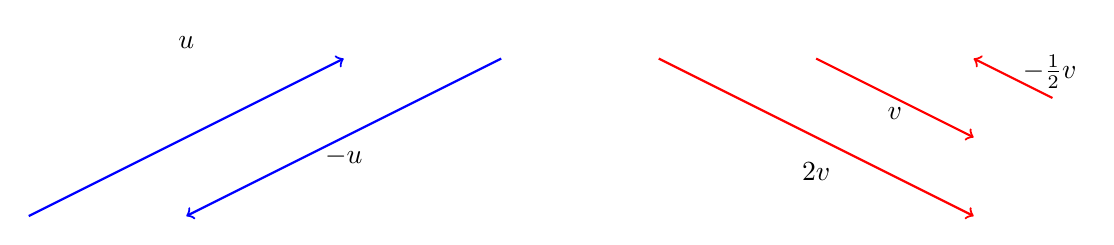
\begin{tikzpicture}[scale=2]
        \draw[->, thick, blue] (0,0)--(2,1);
        \draw[->, thick, blue] (3,1)--(1,0);
        \draw[->, thick, red] (5,1)--(6,0.5);
        \draw[->, thick, red] (6.5,0.75)--(6,1);
        \draw[->, thick, red] (4,1)--(6,0);
        \node[above] at (1,1){$\vect{u}$};
        \node[below] at (2,0.5){$-\vect{u}$};
        \node[below] at (5.5, 0.75){$\vect{v}$};
        \node[above right] at (6.25, 0.75){$-\frac{1}{2}\vect{v}$};
        \node[below] at (5, 0.4){$2\vect{v}$};
      \end{tikzpicture}
